\documentclass{article}
\usepackage[utf8]{inputenc}
\usepackage[margin =1in,includefoot]{geometry}
\usepackage{indentfirst}
\usepackage{graphicx}
\usepackage{float}
\usepackage{caption}
\usepackage{subcaption}
\usepackage[colorlinks=true, linkcolor = blue, urlcolor = cyan]{hyperref}

\title{Assignment 3 - COL334}
\author{Aayush Goyal}
\date{October 2021}

\begin{document}

\maketitle

\tableofcontents

\section{Changing different Congestion Protocols}

\subsection{For each protocol, generate a plot having Congestion window size on the y-axis and
time on the x-axis( till t=30s).}
The following 4 plots have been obtained for the the different congestion protocols that have been mentioned in the assignment statement. The protocols are:
\begin{enumerate}
    \item Tcp NewReno
    \item Tcp HighSpeed
    \item Tcp Veno
    \item Tcp Vegas
\end{enumerate}
\begin{figure}[H]
    \centering
    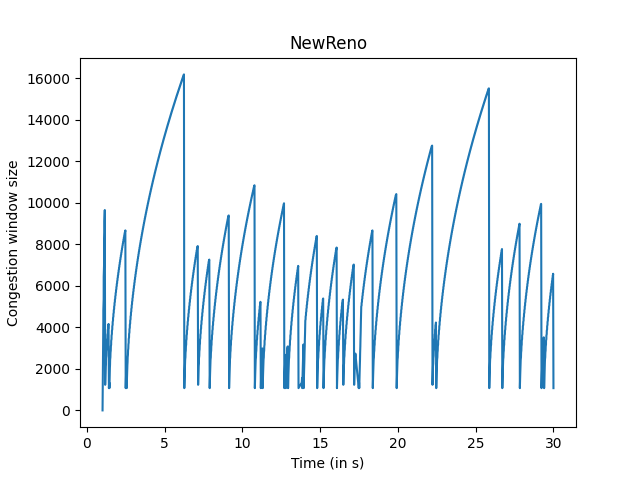
\includegraphics[scale = 0.8]{Q1/outputs/plots/NewReno.png}
    \caption{For the TCP New Reno protocol}
\end{figure}

\begin{figure}[H]
    \centering
    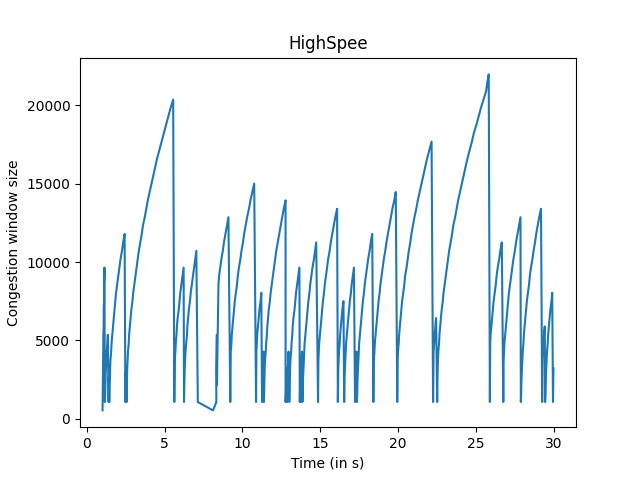
\includegraphics[scale = 0.8]{Q1/outputs/plots/HighSpee.png}
    \caption{For the TCP High Speed protocol}
\end{figure}

\begin{figure}[H]
    \centering
    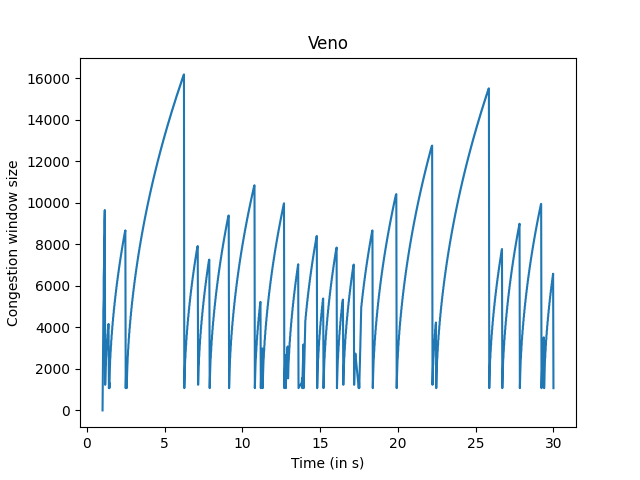
\includegraphics[scale = 0.8]{Q1/outputs/plots/Veno.png}
    \caption{For the TCP Veno protocol}
\end{figure}

\begin{figure}[H]
    \centering
    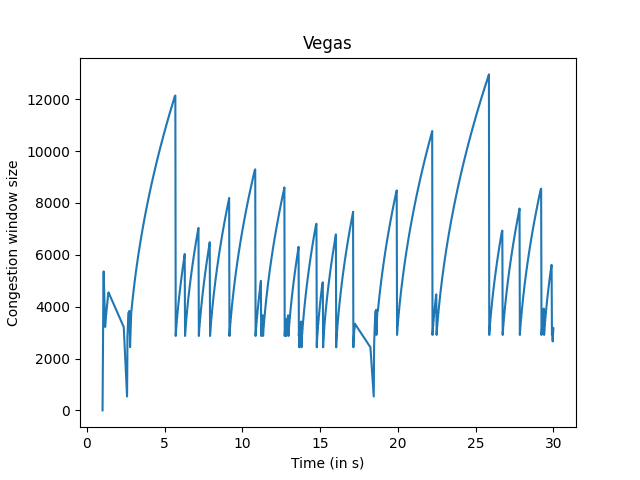
\includegraphics[scale = 0.8]{Q1/outputs/plots/Vegas.png}
    \caption{For the TCP Vegas protocol}
\end{figure}


\subsection{For each protocol, find the number of dropped packets in total. What is your
inference?}
\begin{enumerate}
    \item Tcp NewReno: 38 
    \item Tcp HighSpeed: 38
    \item Tcp Veno: 38
    \item Tcp Vegas: 39
\end{enumerate}

The packet drop happens because of the crowding of the window. We have to drop a packet along with reducing the size of the window to about half. From the data we can see that all of them have almost equal number of packet drops (Tcp Vegas has one more packet drop). The packet drops can be observed from the graph as well. Whenever the size of the congestion window reduces it means there was a packet drop that happened. Generally it happens when we are in the congestion avoidance phase. For all of them it stays true that we can determine the number of packets drops using the number of times there is a decrease in the window size. The only thing different in these protocols is the speed at which the size increases.


\subsection{For each protocol, describe what you observed (4-5 sentences per protocol is
enough). You can talk about the trend you observed in the above plot, the algorithms
they used for different phases etc.}

\subsubsection{TcpNewReno}
\begin{enumerate}
    \item During the slow start phase the size of the congestion window increases by the segment size. Thus we can see that the increase is quite linear in the start, that is the slow start phase.
    \item During the congestion avoidance phase, it increases by $\frac{(seg-size)^2}{cwnd}$. Between that the size of window in reduced to half due to packet drop happening.
    \item The peak of the congestion window size goes to about 16000 and the least value of it remains at around 2000. The average value stays at around the value of 8000.
\end{enumerate}
\subsubsection{TcpHighSpeed}
\begin{enumerate}
    \item This is a different protocol from the otther ones since there is nothing like SlowStart phase and Congestion avoidance phase. 
    \begin{center}
        \textbf{cwnd += a(cwnd)/cwnd}
    \end{center}
    here a(cwnd) is obtanied from the lookup table depending on the value of congestion window size. This can be seen from the huge if else condition given in the code of TcpHighSpeed.
    \item The peak of the congestion window size goes to about 20000 and the least value of it remains at around 0. The average value stays at around the value of 12000.
    \item When compared to the other graphs it can be seen that highspeed is a good method. The maximum is much more and it thus seems that the it will perform better than the other other ones. This is basically because of the absence of the slow start phase.
\end{enumerate}
\subsubsection{TcpVeno}
\begin{enumerate}
    \item During the slow start phase the size of the congestion window increases by the segment size. Thus we can see that the increase is quite linear in the start, that is the slow start phase.
    \item During the congestion avoidance phase, it increases by $\frac{(seg-size)^2}{cwnd}$. Between that the size of window in reduced to half due to packet drop happening.
    \item The Slow start and the congestion phase are both as that of TcpNewReno. This is the reason that both NewReno and Veno has almost similar graph. It includes some good factors of the Vegas also but they are not observable in this small time range.
    \item The peak of the congestion window size goes to about 16000 and the least value of it remains at around 1000. The average value stays at around the value of 8000.
\end{enumerate}
\subsubsection{TcpVegas}
\begin{enumerate}
    \item It keeps a record of the RTT values and compares it to othetrs with the expected throughput. The difference between them provides an estimate of the backlog of the packets. The packet loss increases and decreases linearly with the number of backlog of packets.
    \item The peak of the congestion window size goes to about 12000 and the least value of it remains at around 500. The average least value looks like to stay at around 3000. The average value of the congestion window stays at around 7000. 
    \item This seems to be the least best method among the others since it is actually based on the model that it works to avoid the packet drops. Thus it tries to prevent the drop instead of dropping them.
\end{enumerate}

\section{Changing different Data Rate and Application Data Rate}
\subsection{Plot the congestion window size vs time graph for the TCP connection at different
Channel Data Rates (2Mbps, 4Mbps, 10 Mbps, 20Mbps, 50 Mbps) between N1
and N2. Use Application data rate as 2Mbps. You need to create a plot for each
Channel Data Rate. Explain the trends that you observe.}

\begin{figure}[H]
    \centering
    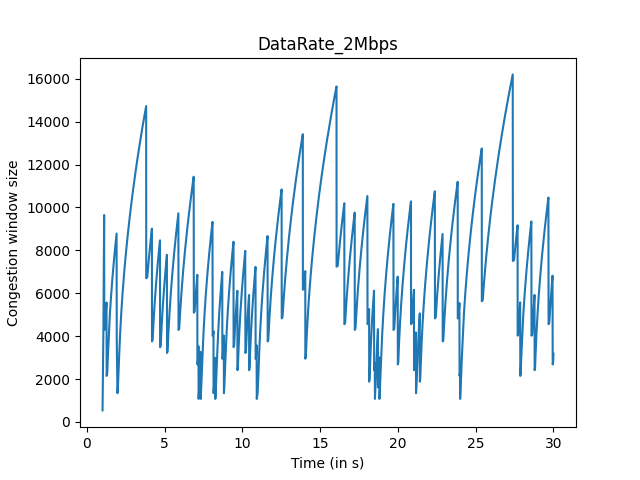
\includegraphics[scale = 0.8]{Q2/outputs/plots/DataRate_2Mbps.png}
    \caption{Data Rate has been fixed to 2Mbps}
\end{figure}

\begin{figure}[H]
    \centering
    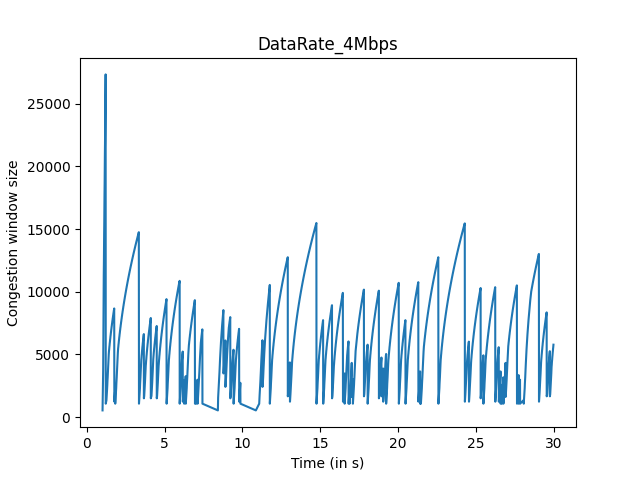
\includegraphics[scale = 0.8]{Q2/outputs/plots/DataRate_4Mbps.png}
    \caption{Data Rate has been fixed to 4Mbps}
\end{figure}

\begin{figure}[H]
    \centering
    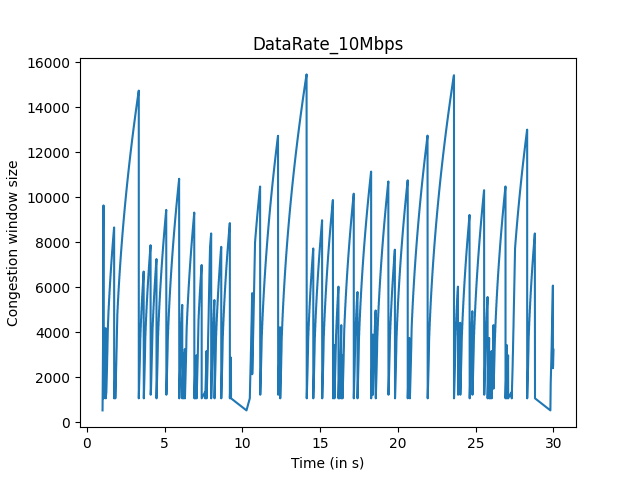
\includegraphics[scale = 0.8]{Q2/outputs/plots/DataRate_10Mbps.png}
    \caption{Data Rate has been fixed to 10Mbps}
\end{figure}

\begin{figure}[H]
    \centering
    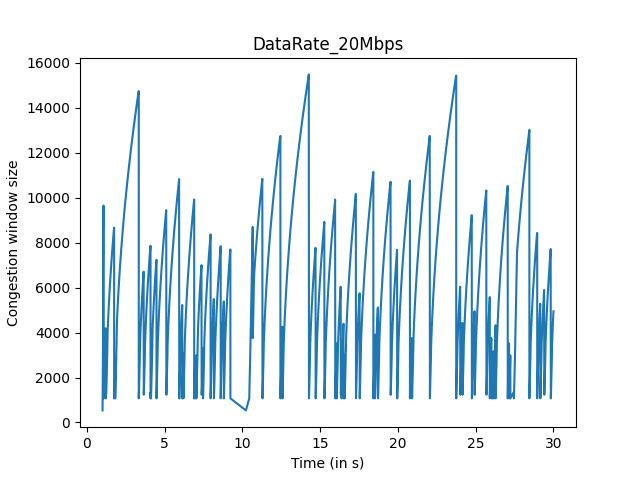
\includegraphics[scale = 0.8]{Q2/outputs/plots/DataRate_20Mbps.png}
    \caption{Data Rate has been fixed to 20Mbps}
\end{figure}

\begin{figure}[H]
    \centering
    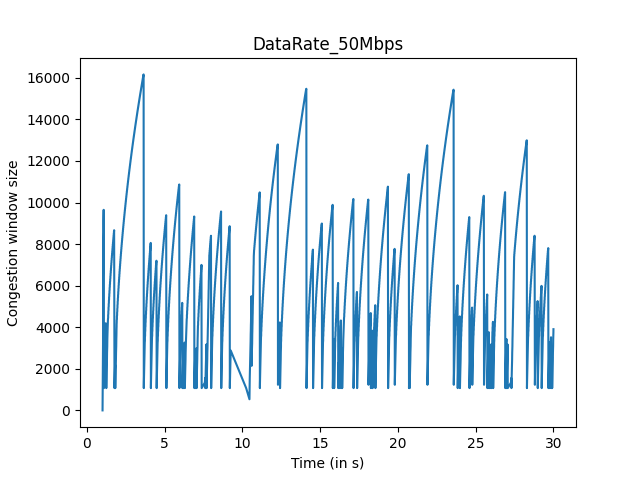
\includegraphics[scale = 0.8]{Q2/outputs/plots/DataRate_50Mbps.png}
    \caption{Data Rate has been fixed to 50Mbps}
\end{figure}


Larger variation in the congestion window for larger channel rate is due to the high frequence of packet drops. We can see that amount of variation in the congestion window per second increases. This will happen as it becomes more easy to transmit more number of packets over the link. Thus we can also see that the last three graphs are almost same due to above reason.


\subsection{Plot the congestion window size vs time graph for the TCP connection at different
Application Data Rates (0.5 Mbps, 1Mbps, 2Mbps, 4Mbps, 10 Mbps). Use Channel
data rate between N1 and N2 as 6 Mbps. You need to create a plot for each
Application data rate. Explain the trends that you observe.}

\begin{figure}[H]
    \centering
    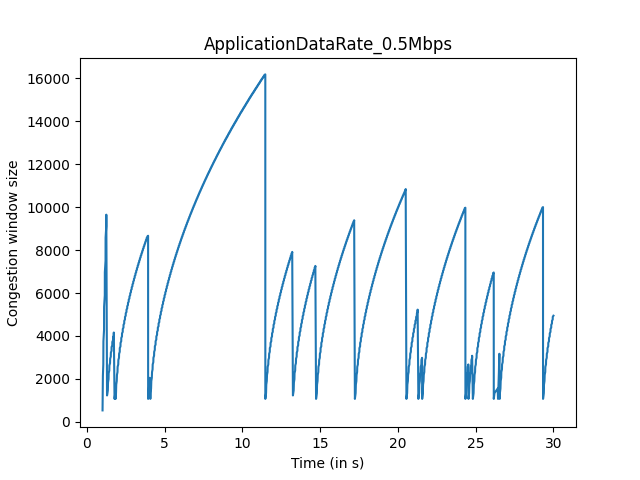
\includegraphics[scale = 0.8]{Q2/outputs/plots/ApplicationDataRate_0.5Mbps.png}
    \caption{Application Data Rate has been fixed to 0.5Mbps}
\end{figure}

\begin{figure}[H]
    \centering
    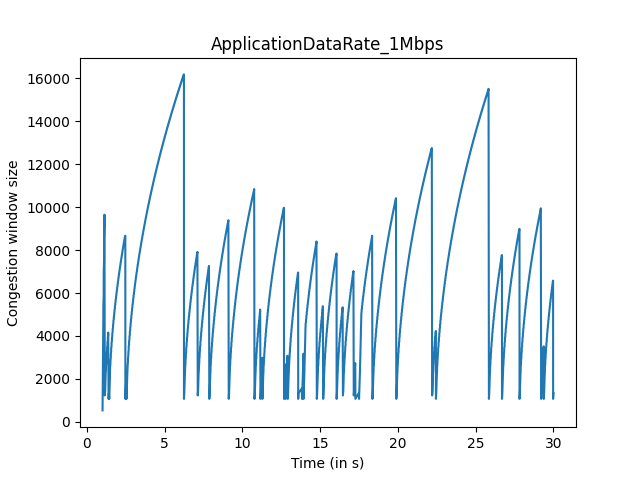
\includegraphics[scale = 0.8]{Q2/outputs/plots/ApplicationDataRate_1Mbps.png}
    \caption{Application Data Rate has been fixed to 1Mbps}
\end{figure}

\begin{figure}[H]
    \centering
    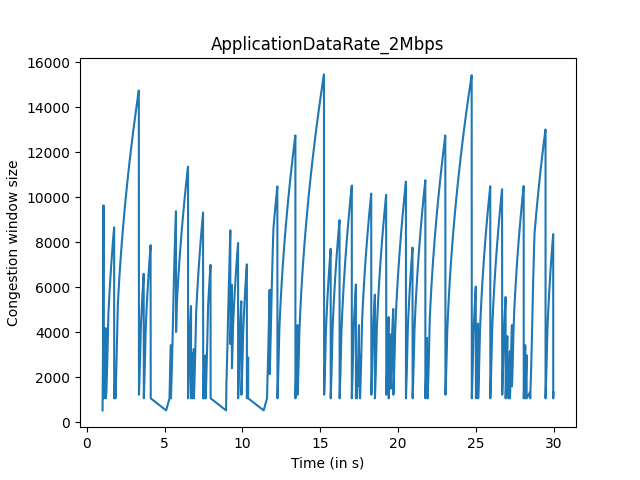
\includegraphics[scale = 0.8]{Q2/outputs/plots/ApplicationDataRate_2Mbps.png}
    \caption{Application Data Rate has been fixed to 2Mbps}
\end{figure}

\begin{figure}[H]
    \centering
    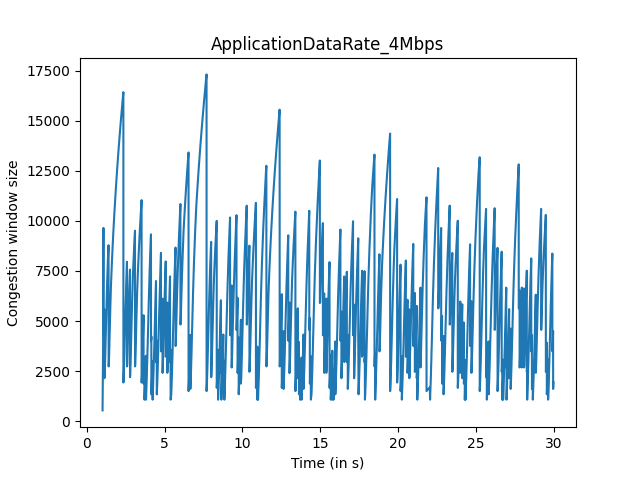
\includegraphics[scale = 0.8]{Q2/outputs/plots/ApplicationDataRate_4Mbps.png}
    \caption{Application Data Rate has been fixed to 4Mbps}
\end{figure}

\begin{figure}[H]
    \centering
    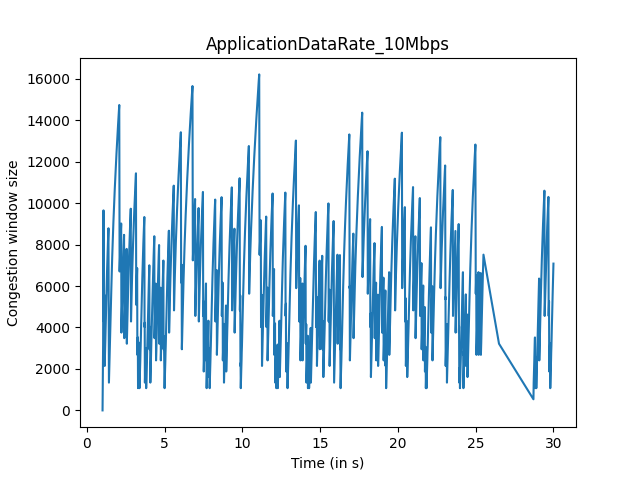
\includegraphics[scale = 0.8]{Q2/outputs/plots/ApplicationDataRate_10Mbps.png}
    \caption{Application Data Rate has been fixed to 10Mbps}
\end{figure}

Drop rate increases for larger application rates. This can be seen from the following obseravtions. For smaller application rates, the congestion avoidance phase is for a longer time and as the the application rate increases we can see that it shift towards the slow start phase. For the larger application rate there is a region of lesser window size. Thus we can conculde that we need to keep a slower application rate in order to accomodate the the congestion in network.

\section{Implementing TcpNewRenoCSE}

The files have been included with the submission which contain the code for SlowStart and Congestion Avoidance. How to compile them is given in the README.md

\subsection{Plot Congestion window size vs time (from t=1 to t=30 seconds)}

\begin{figure}[H]
    \centering
    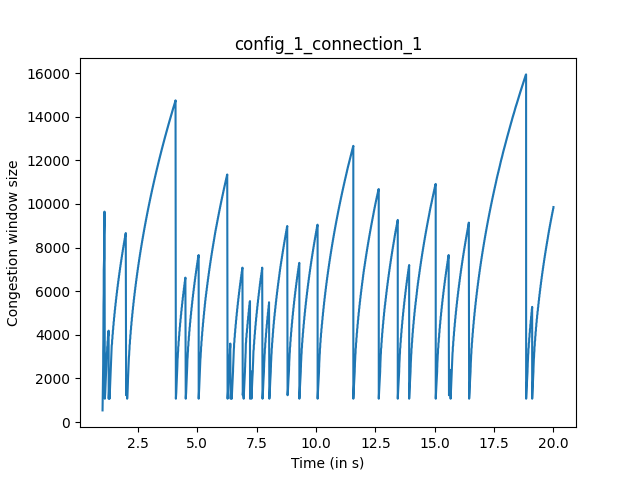
\includegraphics[scale = 0.8]{Q3/outputs/plots/config_1_connection_1.png}
    \caption{Plot for Configuration 1 and Connection 1}
\end{figure}

\begin{figure}[H]
    \centering
    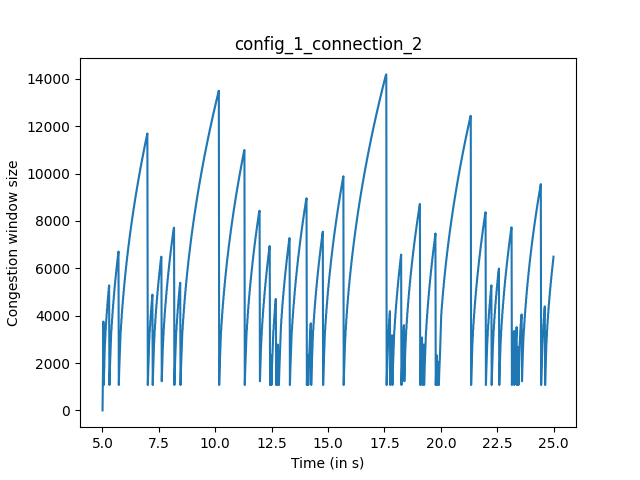
\includegraphics[scale = 0.8]{Q3/outputs/plots/config_1_connection_2.png}
    \caption{Plot for Configuration 1 and Connection 2}
\end{figure}

\begin{figure}[H]
    \centering
    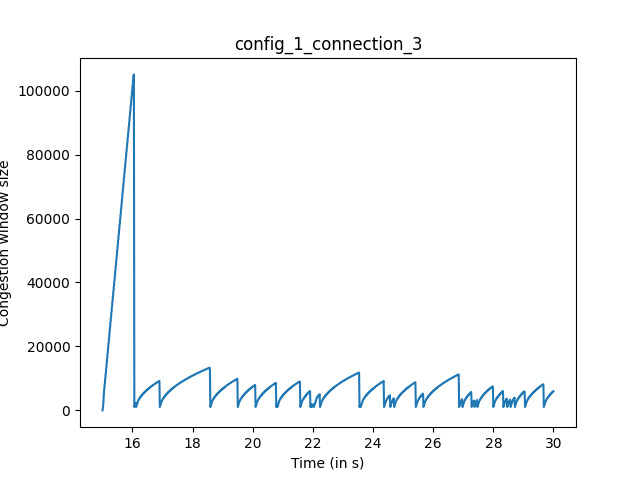
\includegraphics[scale = 0.8]{Q3/outputs/plots/config_1_connection_3.png}
    \caption{Plot for Configuration 1 and Connection 3}
\end{figure}

\begin{figure}[H]
    \centering
    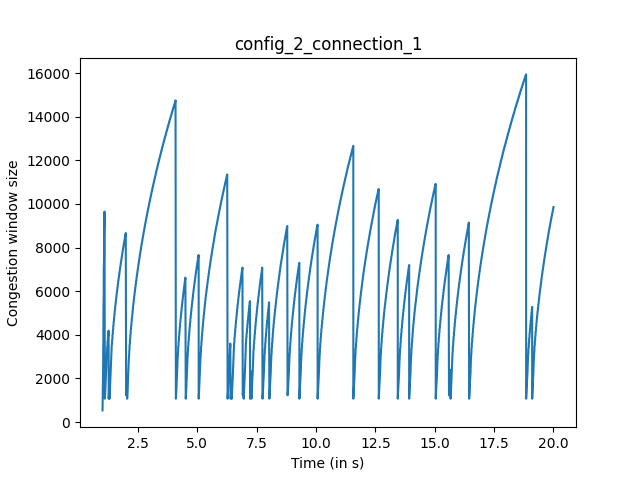
\includegraphics[scale = 0.8]{Q3/outputs/plots/config_2_connection_1.png}
    \caption{Plot for Configuration 2 and Connection 1}
\end{figure}

\begin{figure}[H]
    \centering
    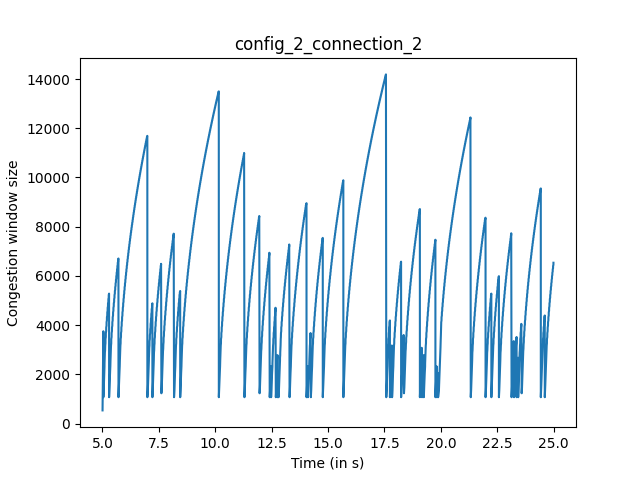
\includegraphics[scale = 0.8]{Q3/outputs/plots/config_2_connection_2.png}
    \caption{Plot for Configuration 2 and Connection 2}
\end{figure}

\begin{figure}[H]
    \centering
    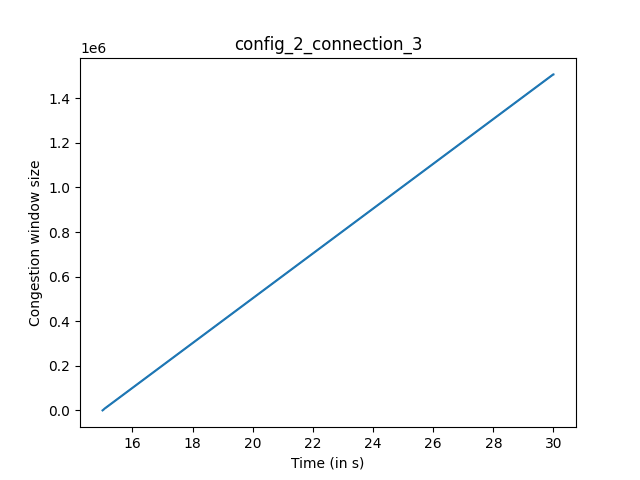
\includegraphics[scale = 0.8]{Q3/outputs/plots/config_2_connection_3.png}
    \caption{Plot for Configuration 2 and Connection 3}
\end{figure}

\begin{figure}[H]
    \centering
    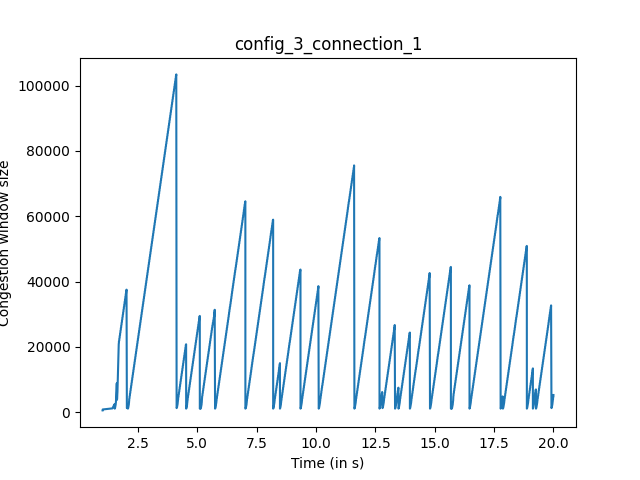
\includegraphics[scale = 0.8]{Q3/outputs/plots/config_3_connection_1.png}
    \caption{Plot for Configuration 3 and Connection 1}
\end{figure}


\begin{figure}[H]
    \centering
    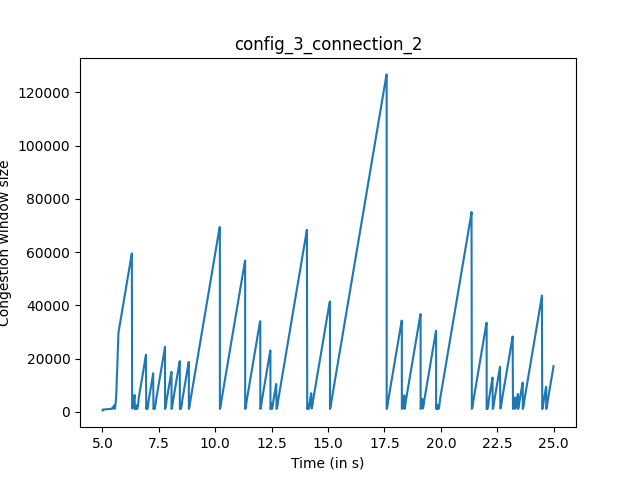
\includegraphics[scale = 0.8]{Q3/outputs/plots/config_3_connection_2.png}
    \caption{Plot for Configuration 3 and Connection 2}
\end{figure}

\begin{figure}[H]
    \centering
    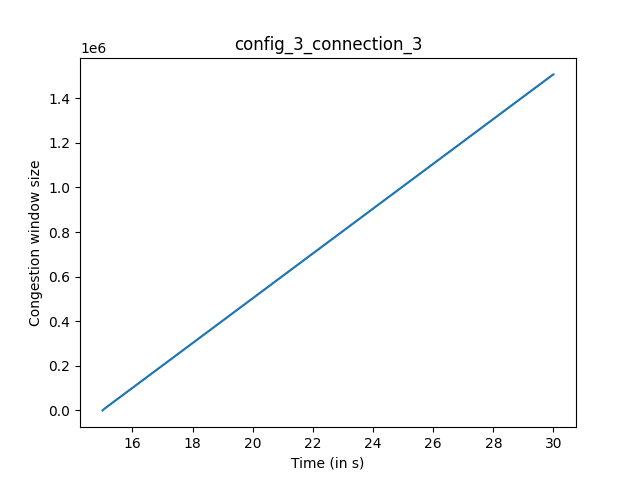
\includegraphics[scale = 0.8]{Q3/outputs/plots/config_3_connection_3.png}
    \caption{Plot for Configuration 3 and Connection 3}
\end{figure}

\subsection{Report the total number of dropped packets in each scenario.}

For this part I have made 2 errror models. In the updated assignment statement it is written that we have to just report only 3 values, one for each Configuration.

\begin{enumerate}
    \item Configuration 1: 113
    \item Configuration 2: 112
    \item Configuration 3: 110
\end{enumerate}

\subsection{How does the congestion avoidance phase vary on the same sender when using
TCPNewRenoCSE vs TCPNewReno? Explain the observed trends. How does it
impact the entire network?}

% TODO: Writing what is asked in the above part

\begin{itemize}
    \item We can notice that the average congestion window size is higher Whenever we use the TcpNewRenoCSE instead of TcpNewReno for a single connection. 
    \item There happens a large number of packet drops on the first link for both of the models and thus we can see that both slow start and congestion avoidance states are achieved.
    \item In configuration 1 and 3, for the connection 1 and 2, the congestion window size achieved much higher values as comapred to the configuration 2.
    \item In cinfiguration 1 and 3, the proticol largely reamins in the congestion avoidance phase which leads to relatively large congestion window size.
    \item In case of configuration 3, for connection 3 the large increase in the congestion window size is due to the slow start phase. When it shifts to congestion avoidance there is a linear increase. 
\end{itemize}


\section{Directory Structure}

As specified in the problem statement. I have submitted a plot.py, the instructions of how to use it have been given in the README.md. Apart from that the outputs have been stored in the following format, in the outputs folder of each question:
\begin{itemize}
    \item dropped: It contains the information regarding which how many packets have been dropped for a particular part
    \item toplot: This contains the time vs the old congestion window size vs the new window size. My plotting script takes all the files present in this and plots them.
    \item plots: This contains the plots. Look at the titles of the plots for information about them.
\end{itemize}
Further instructions on how to run have been given in the \textbf{README.md} in a well detailed manner.
\end{document}
